\chapter{Numerical Results}

In this section, we will show our approximation results for square root mean-reverting model and one heston one CEV model, we expand this method with corrective terms up to 3. We use a symbolic library of \footnote{Codes used for this paper can be accessed through my \href{https://github.com/ywang408/master-thesis-code}{github}}{python} \href{https://www.sympy.org/en/index.html}{sympy} to do expansions, and Monte Carlo simulations with 200 steps and 100000 paths as our benchmark because there's no existing pricing formulas for these models. We use two kinds of figures to evaluate the accuracy of our results, the first kind is the direct comparison between benchmarks and our approximation results, the second one is the relative differences between benchmarks and our results. Besides, we also attach detailed results in the Appendix \ref{mrcev}.

\section{Volatility option prices under mean-reverting CEV model}

For options under mean-reverting CEV model, generally we use the same mean-reverting parameters as \cite{grunbichler_valuing_1996} used in his model, the parameters are $\kappa=4$, $\theta=2$, $K=0.15$. Besides, we set the nuisance parameter $\sigma_0 = \sigma_{\text{CEV}} v_0^{\gamma-\frac{1}{2}}$, where $v_0$ is the initial value of volatility. We test our approximation method with different constant elasticity parameters, the main idea of setting these parameters is that for small $\gamma$, which enlarges the importance of $v(t)$ in the CEV part, we use a small $\sigma$; Whereas for large $\gamma$ we set a large $\sigma$. 

For figure \ref{price comparison1} and figure \ref{price comparison2},our parameters are $\sigma=0.15$, $\gamma=0.3$, and with different maturities $T=0.3$, $T=0.5$. We can find that our results with corrective terms $N=3$ are very accurate; Figure \ref{price diff1} and figure \ref{price diff2} use the same parameters but show the relative error with different corrective terms. We can find that the results with highest corrective terms outperform other results, which proves that keep applying Ito-Taylor expansions on the mis-pricing formula can create increasingly improved refinements and provide us with highly accurate results.

\begin{figure}[!tbp]
    \centering
    \subfloat[price comparison]{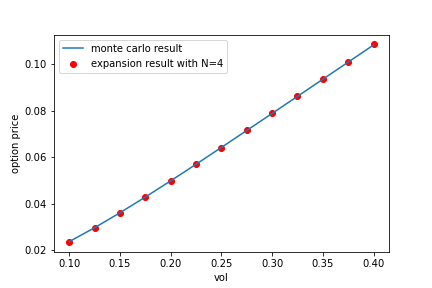
\includegraphics[width=0.5\textwidth]{./figures/T=0.3,K=0.15, kappa=4,m=0.2, sigma=0.15, gamma=0.3.csv price.png}\label{price comparison1}}
    \hfill
    \subfloat[relative error]{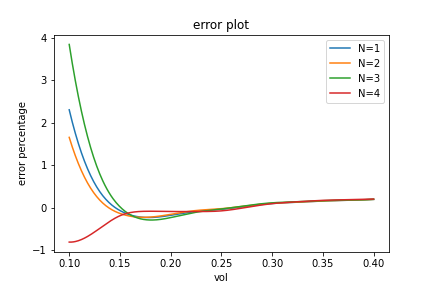
\includegraphics[width=0.5\textwidth]{./figures/T=0.3,K=0.15, kappa=4,m=0.2, sigma=0.15, gamma=0.3.csv error.png}\label{price diff1}}
    \caption{Parameters are $T=0.3,K=0.15, \kappa=4,\theta=0.2, \sigma=0.15, \gamma=0.3$}
  \end{figure}

\begin{figure}[!tbp]
  \centering
  \subfloat[price comparison]{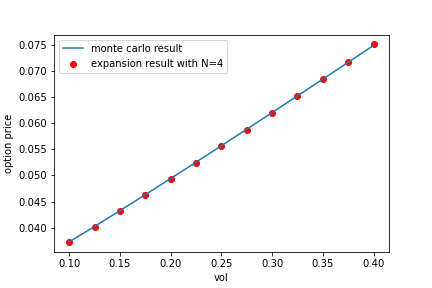
\includegraphics[width=0.5\textwidth]{./figures/T=0.5,K=0.15, kappa=4,m=0.2, sigma=0.15, gamma=0.3.csv price.png}\label{price comparison2}}
  \hfill
  \subfloat[relative error]{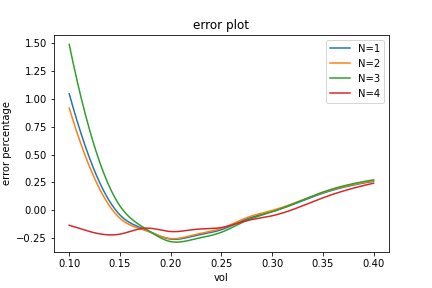
\includegraphics[width=0.5\textwidth]{./figures/T=0.5,K=0.15, kappa=4,m=0.2, sigma=0.15, gamma=0.3.csv error.png}\label{price diff2}}
  \caption{Parameters are $T=0.5,K=0.15, \kappa=4,\theta=0.2, \sigma=0.15, \gamma=0.3$}
\end{figure}

Parameters for figure \ref{price comparison3} and figure \ref{price comparison4},our parameters are $\sigma=0.6$, $\gamma=0.75$, and with different maturities $T=0.3$, $T=0.5$. Similarly, our method still provide accurate results.

\begin{figure}[!tbp]
  \centering
  \subfloat[price comparison]{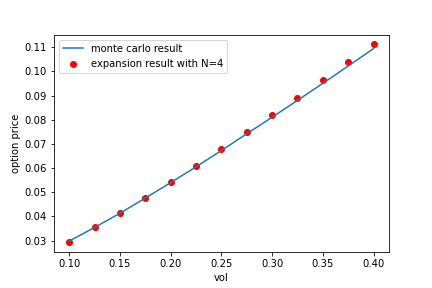
\includegraphics[width=0.5\textwidth]{./figures/T=0.3,K=0.15, kappa=4,m=0.2, sigma=0.6, gamma=0.75.csv price.png}\label{price comparison3}}
  \hfill
  \subfloat[relative error]{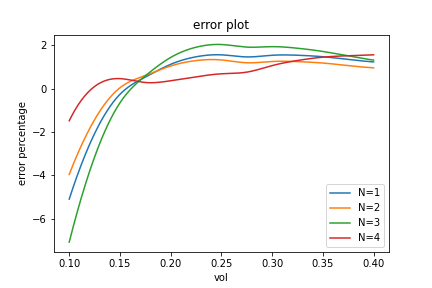
\includegraphics[width=0.5\textwidth]{./figures/T=0.3,K=0.15, kappa=4,m=0.2, sigma=0.6, gamma=0.75.csv error.png}\label{price diff3}}
  \caption{Parameters are $T=0.3,K=0.15, \kappa=4,\theta=0.2, \sigma=0.6, \gamma=0.75$}
\end{figure}

\begin{figure}[!tbp]
    \centering
    \subfloat[price comparison]{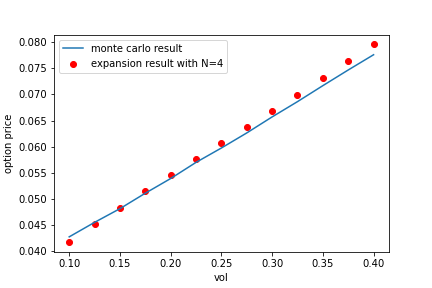
\includegraphics[width=0.5\textwidth]{./figures/T=0.5,K=0.15, kappa=4,m=0.2, sigma=0.6, gamma=0.75.csv price.png}\label{price comparison4}}
    \hfill
    \subfloat[relative error]{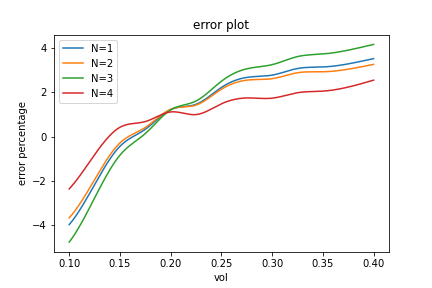
\includegraphics[width=0.5\textwidth]{./figures/T=0.5,K=0.15, kappa=4,m=0.2, sigma=0.6, gamma=0.75.csv error.png}\label{price diff4}}
    \caption{Parameters are $T=0.5,K=0.15, \kappa=4,\theta=0.2, \sigma=0.6, \gamma=0.75$}
\end{figure}

One may observe that when KM use Black-Scholes model as auxiliary model to price options under Heston model, for deep in-the-money options, relative error always converge to 0 no matter how many corrective terms are applied. That is because in that case, delta of option is very close to 1 and vega are close to 0, which means option prices are mainly driven by underlying stocks' prices and volatility has no influence on option prices. Besides, gamma of options is also close to 0, meaning that their mis-pricing terms don't affect option prices at all. As a result, their figures show that all results' relative errors are converging to 0 as stock price increases.

However, in our model, underlying assets follow mean-reverting CEV model. \cite{grunbichler_valuing_1996} mention that when volatility $V$ is above its long-term mean, mean-reversion property implies the expected future value of V will be lower than its current value, making the expected payoff for a volatility call can be less than its current intrinsic value. Recall that before we set $\sigma_0 = \sigma_{\text{CEV}}v_0^{\gamma-\frac{1}{2}}$, that is 

$$
\begin{cases}
  d V_t=\kappa(m - V_t) d t+\sigma_{\text{CEV}} V^{\gamma}_t d W_t &\text{true model}\\
  d V_t=\kappa(m - V_t) d t+\sigma_{\text{CEV}}v_0^{\gamma-\frac{1}{2}} \sqrt{V}_t d W_t &\text{auxiliary model}
\end{cases}
$$

\noindent Obviously when $V$ is large, $\sigma_{\text{CEV}} V^{\gamma}_t > \sigma_{\text{CEV}}v_0^{\gamma-\frac{1}{2}} \sqrt{V}_t$, causing the loss of accuracy. It gives an explanation why the relative error our method is slightly larger than 0.